
\documentclass{beamer} 
\usetheme{Singapore}
\usecolortheme{seagull}

\usepackage[utf8]{inputenc}
\usepackage[portuguese]{babel}
\usepackage{lmodern}
\usepackage[absolute,overlay]{textpos} 
\newenvironment{reference}[2]{% 
  \begin{textblock*}{\textwidth}(#1,#2) 
      \footnotesize\it\bgroup\color{red!50!black}}{\egroup\end{textblock*}} 
\title{Introdução a segurança em sistemas de informação}
\author[Lopez. V.L.O, Winck. A. T]{Víctor Orozco, Dr. Ana Trindade Winck}
\institute[UFSM]{
  Centro de Tecnologia \\
  Universidade Federal de Santa Maria
}
\date{\today}

\begin{document}
\begin{frame}[Plain]
\titlepage
\end{frame}

\begin{frame}{Objetivos da aula}
\begin{itemize}
\item Apresentar uma visão geral da grande área de segurança da informação
\item Identificar princípios básicos de segurança
\item Discutir um modelo genérico de segurança de informação
\end{itemize}
\end{frame}

\begin{frame}
\frametitle{Roteiro}
\tableofcontents
\end{frame} 

\section{Visão geral}
\begin{frame}{Segurança}
\begin{figure}[tbph]
\centering

\includegraphics[width=0.3\linewidth]{./question}
\label{fig:question}
\end{figure}
\end{frame}

\begin{frame}{Segurança}
\begin{itemize}
\item A segurança é um dos mais antigos problemas que governos, organizações comerciais e quase todas as pessoas tem de enfrentar
\item Pode-se definir a segurança como a percepção de estar protegido contra riscos, perigos ou perdas.
\end{itemize}
\end{frame}

\begin{frame}{Segurança}
\begin{itemize}
\item Em um sentido amplio a segurança significa proteger os nossos ativos
\begin{itemize}
\item Proteger os nossos sistemas contra atacantes
\item Proteger o nosso prédio contra desastres naturais
\item Proteger a nossa carteira de roubos na boate
\end{itemize}
\end{itemize}
\end{frame}

\begin{frame}{Segurança}
\begin{itemize}
\item Dependendo do contexto assim tem que ser as medidas de segurança
\begin{itemize}
\item Ativos físicos: Computadores, carros
\item Ativos lógicos: Arquivos de dados, código fonte de aplicativos
\item Ativos humanos: Seres humanos a base de qualquer negocio
\end{itemize}
\end{itemize}
\end{frame}



\begin{frame}{Segurança em SI}
\begin{itemize}
\item Segurança SI = Proteger sistemas de informação e a informação mesma de acesso não autorizado, uso, divulgação, interrupção, modificação ou destruição
\end{itemize}
\end{frame}

\begin{frame}{Segurança em SI}
\begin{itemize}
\item Conceito que se torna cada vez mais presente em muitos aspectos da nossa sociedade
\item Embora a tecnologia nos permite ser mais produtivos, ela também carrega consigo uma série de questões de segurança
\item A introdução de sistemas de informação na industria tem aumentado o problema de segurança ainda mais
\item Se a informação sobre os sistemas utilizados pelos nossos empregadores ou nossos bancos fica exposta a um atacante, as consequências podem ser devastadoras
\end{itemize}
\end{frame}


\begin{frame}{Assegurando Informação}
``O único sistema realmente seguro é aquele que está desligado, dentro dum bloco de concreto com guardas armados, e mesmo assim eu tenho minhas dúvidas''\cite{andress2011the}.
\end{frame}

\begin{frame}{Assegurando Informação}
\begin{itemize}
\item Quanto mais aumentamos o nível de segurança, geralmente diminui o nível de produtividade
\item Devemos também considerar como o nível de segurança refere-se o valor do item que está sendo assegurado
\item Podemos construir uma instalação militar cercada por cães assassinos  . . . mas não faz sentido se o ativo a proteger for a lista de compras do mercado.
\end{itemize}
\end{frame}

\begin{frame}{Assegurando Informação}
\begin{itemize}
\item Definir um nível aceitável de segurança é um processo subjectivo
\item Técnica generalizada: Definir uma lista dos ativos onde somos vulneráveis (sempre vai ter alguma coisa a mais)
\item Alguns regulamentos tentam definir o que proteger, ou pelo menos alguns dos passos que uma organização deve tomar para ser ``seguro''.
\end{itemize}
\end{frame}

\begin{frame}{Assegurando Informação}
\begin{itemize}
\item Como pode-se definir esse listado?
\item Listando nossos ativos e verificando se eles apresentam características seguras de acordo a algum modelo estandardizado
\end{itemize}
\end{frame}


\section{Modelo geral de segurança}
\begin{frame}{Modelo CID}
\begin{figure}[tbph]
\centering
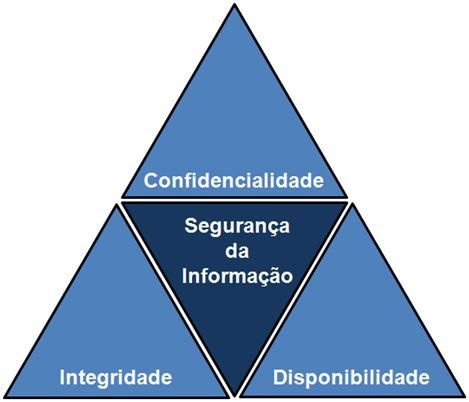
\includegraphics[width=0.5\linewidth]{./cia1}
\label{fig:cia}
\end{figure}
\end{frame}

\begin{frame}{Modelo CID - Confidencialidade}
Nossa capacidade de proteger nossos dados daqueles que não estão autorizados a ver eles.
\end{frame}

\begin{frame}{Modelo CID - Confidencialidade}
\begin{itemize}
\item Password do nosso computador
\item Registo bancário
\item ? 
\end{itemize}
\end{frame}

\begin{frame}{Modelo CID - Integridade}
A capacidade de impedir os nossos dados sejam alteradas numa forma não autorizada ou indesejável.
\end{frame}

\begin{frame}{Modelo CID - Integridade}
\begin{itemize}
\item Sistema de arquivos Windows que separa e protege o acesso aos arquivos de um usuário para outro
\item ?
\end{itemize}
\end{frame}

\begin{frame}{Modelo CID - Disponibilidade}
A capacidade de acessar aos dados quando precisamos deles.
\end{frame}

\begin{frame}{Modelo CID - Disponibilidade}
\begin{itemize}
\item Sobrecarga mal intencionada nos servidores do nosso banco
\item ?
\end{itemize}
\end{frame}

\begin{frame}{Modelo Parkeriano -2002-}
\begin{figure}[tbph]
\centering
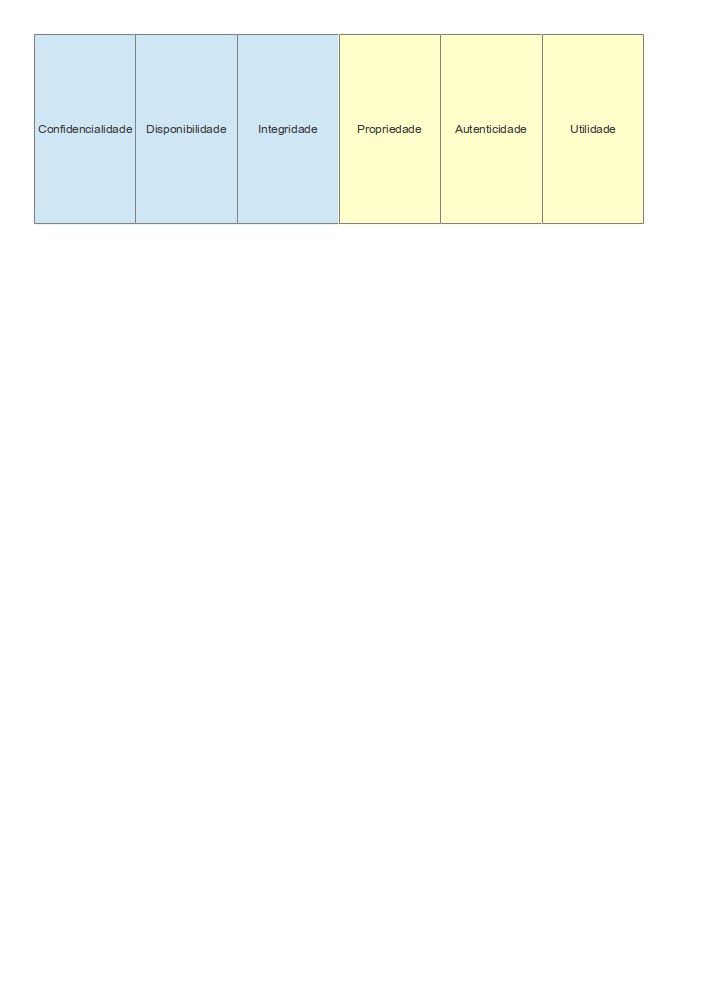
\includegraphics[width=0.90\linewidth]{./parkerian.png}
\label{fig:parkeran}
\end{figure}
\end{frame}

\begin{frame}{Modelo Parkeriano}
\begin{itemize}
\item Propriedade - A disponibilidade física donde a informação tem sido guardada
\item Autenticidade - A atribuição adequada quanto ao proprietário ou criador dos dados em questão
\item Utilidade - Quão útil são os dados e suas características para nós
\end{itemize}
\end{frame}

\section{Ataques}
\begin{frame}{Ataques}
\begin{itemize}
\item Os sistemas de informação podem enfrentar ataques desde uma grande variedade de abordagens e ângulos
\item Os ataques podem ser classificados de acordo com o tipo de ataque que ele representa, o risco que o ataque representa, e os controles podemos usar para mitigar eles
\item Cada ataque pode afetar um ou mais princípios CID
\end{itemize}
\end{frame}


\begin{frame}{Ataques}
\begin{figure}[tbph]
\centering
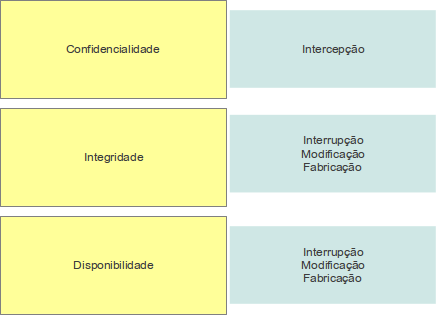
\includegraphics[width=0.70\linewidth]{./atacks.png}
\label{fig:atacks}
\end{figure}
\end{frame}

\begin{frame}{Ataques - Intercepção}
\begin{itemize}
\item Permitem que usuários não autorizados acessem os nossos dados, aplicações, ou ambientes, e são principalmente um ataque contra a confidencialidade (chaves de acesso).
\item Exemplos: Visualização ou copia de arquivos não autorizados, espionagem em conversas, ler e-mail
\item Corretamente executados, ataques de interceptação podem ser muito difíceis de detectar.
\end{itemize}
\end{frame}

\begin{frame}{Ataques - Interrupção}
\begin{itemize}
\item Atacam ativos visando tornar eles inutilizáveis ou indisponíveis para uso, de forma temporária ou permanente.
\item Exemplos: Ataques de denegação de serviço (disponibilidade), sobrecarga aos bancos de dados (disponibilidades+integridade), 
\item Modificação
\item Fabricação
\end{itemize}
\end{frame}

\begin{frame}{Ataques - Modificação}
\begin{itemize}
\item São todos aqueles que mexem na informação.
\item Exemplos: Acesso não autorizado a arquivos (integridade), acesso a arquivos de configuração de serviços (integridade+disponibilidade)
\end{itemize}
\end{frame}

\begin{frame}{Ataques - Fabricação}
\begin{itemize}
\item Geração de dados, processos, comunicações ou outras atividades similares com um sistema de
\item Exemplo: Criação de informações falsas no banco de dados (integridade ou integridade+disponibilidade)
\item São considerados maioritariamente como ataques na integridade, mas dependendo da quantidade dos dados podem ser também ataques de disponibilidade
\end{itemize}
\end{frame}

\section{Referencias}
\begin{frame}[allowframebreaks]{Referencias}
    \bibliographystyle{sbc}
    \bibliography{small}
\end{frame}
\end{document}